\chapter{Implémentation technique dans Collec}

Collec est un logiciel de gestion de collections d'échantillons, dont l'objectif principal vise à faciliter la recherche d'un échantillon stocké ou de récupérer les informations générales le concernant.

Écrit en PHP, les données sont stockées dans une base de données PostgreSQL. Le code de l'application est disponible à l'adresse \url{https://gitlab.com/Irstea/collec}. Il est disponible sous licence AGPL.

Le logiciel est bâti sur un modèle MVC, tous les accès étant gérés par l'appel à des modules déclarés dans un fichier spécifique. 

La gestion matérielle des échantillons de laboratoire (ou d'expérimentations scientifiques) est une fonctionnalité largement demandée, mais peu couverte jusqu'à présent par les logiciels disponibles, et particulièrement dans le domaine de l'\textit{Open Source}. Collec, dont la première version remonte à l'automne 2016, fait l'objet d'un réel intérêt de la part de la communauté scientifique, ses fonctionnalités et sa facilité d'utilisation le rendant attractif.

Toutefois, il n'est pas conçu comme un système global de gestion de données à la fois techniques -- stockage des échantillons -- et de résultats d'analyse par exemple (pas d'informations métiers complexes\footnote{Dans la pratique, à partir de la version 1.1, il est possible de renseigner quelques informations métiers, mais de manière relativement frustre et sans permettre la complexité des actions envisageables avec des bases de données dédiées.}).
Il n'est pas non plus prévu de mettre en place un hébergement centralisé qui permettrait de gérer tous les échantillons de la sphère de recherche.

\textit{A contrario}, cette organisation permet de créer autant d'instances que néces\-saires, notamment pour gérer des saisies en mode décentralisé (bateau partant en campagne de sondage dans les mers du Sud, collecte d'échantillons depuis des zones non couvertes par Internet, par exemple).

Cette souplesse nécessite de prévoir des mécanismes soit d'interrogation de diverses instances, soit de récupération des informations concernant des échantillons provenant d'autres bases de données. 

\section{Transformation des URL et appel aux modules}
Les URL conviviales sont transformées en noms de modules, selon le fonctionnement suivant :
\begin{itemize}
\item les trois premiers éléments de l'adresse sont fusionnés;
\item si le quatrième élément est présent, il est stocké dans la variable de requête \textit{\$id}, et :
\begin{itemize}
\item si la requête est de type GET, le module est suffixé par \textit{Display};
\item si la requête est de type POST, le module est suffixé par \textit{Write}\footnote{Dans la version actuelle, l'écriture depuis une instance distante n'est pas implémentée};
\end{itemize}
\item sinon, le module est suffixé par \textit{List}.
\end{itemize}

Les modules doivent être décrits, comme les autres, dans le fichier \textit{param/actions.xml}, et sont exécutés selon le fonctionnement classique de l'application.

\section{Emplacement du code}
Le code spécifique des modules doit être stocké dans le dossier \textit{modules}, en respectant l'arborescence des URL conviviales, par exemple, pour l'adresse \textit{http://collec.local/sw/v1/sample}, dans le sous-dossier \textit{sw/v1}.


\subsection{Données d'identification des instances distantes}
\label{table_instance}

Pour identifier les instances clientes, la table \textit{instance} contient les données suivantes :
\begin{itemize}
\item le nom de l'instance;
\item l'url de l'instance ;
\item le nom d'un contact;
\item son mail;
\item le code attribué en conservant les 8 premiers caractères du calcul d'empreintes sha256 de l'url;
\item le secret, généré de manière cryptographique ;
\item le type d'instance (cliente ou serveur);
\item la date de fin d'autorisation d'accès, par défaut, fixée à 5 ans.
\end{itemize}

Si une instance est à la fois cliente et serveur, deux lignes devront être créées, l'une pour chaque sens de communication. Cela permet de maintenir des secrets différents pour chaque canal.

Pour les instances \og serveurs\fg{}, une table complémentaire permet d'indiquer les URI des services web disponibles :
\begin{itemize}
\item le type du service web;
\item l'URI correspondante;
\item mécanisme d'identification.
\end{itemize}

Afin de permettre les échanges automatisés des paramètres entre les serveurs, le type du service web (son identifiant) doit impérativement respecter le contenu de cette table :
\begin{longtable}{|c|>{\raggedright\arraybackslash}p{10cm}|}
\hline 
Code & Service web  \\ 
\hline \endhead
1 & Liste des tables de paramètres utilisables \\
\hline
2 & Contenu d'une table de paramètres \\
\hline
3 & Recherche d'échantillons \\
\hline
4 & Consultation d'un échantillon \\
\hline
5 & Consultation d'une liste d'échantillons\\
\hline

\end{longtable}

\subsection{Structure des tables correspondantes}

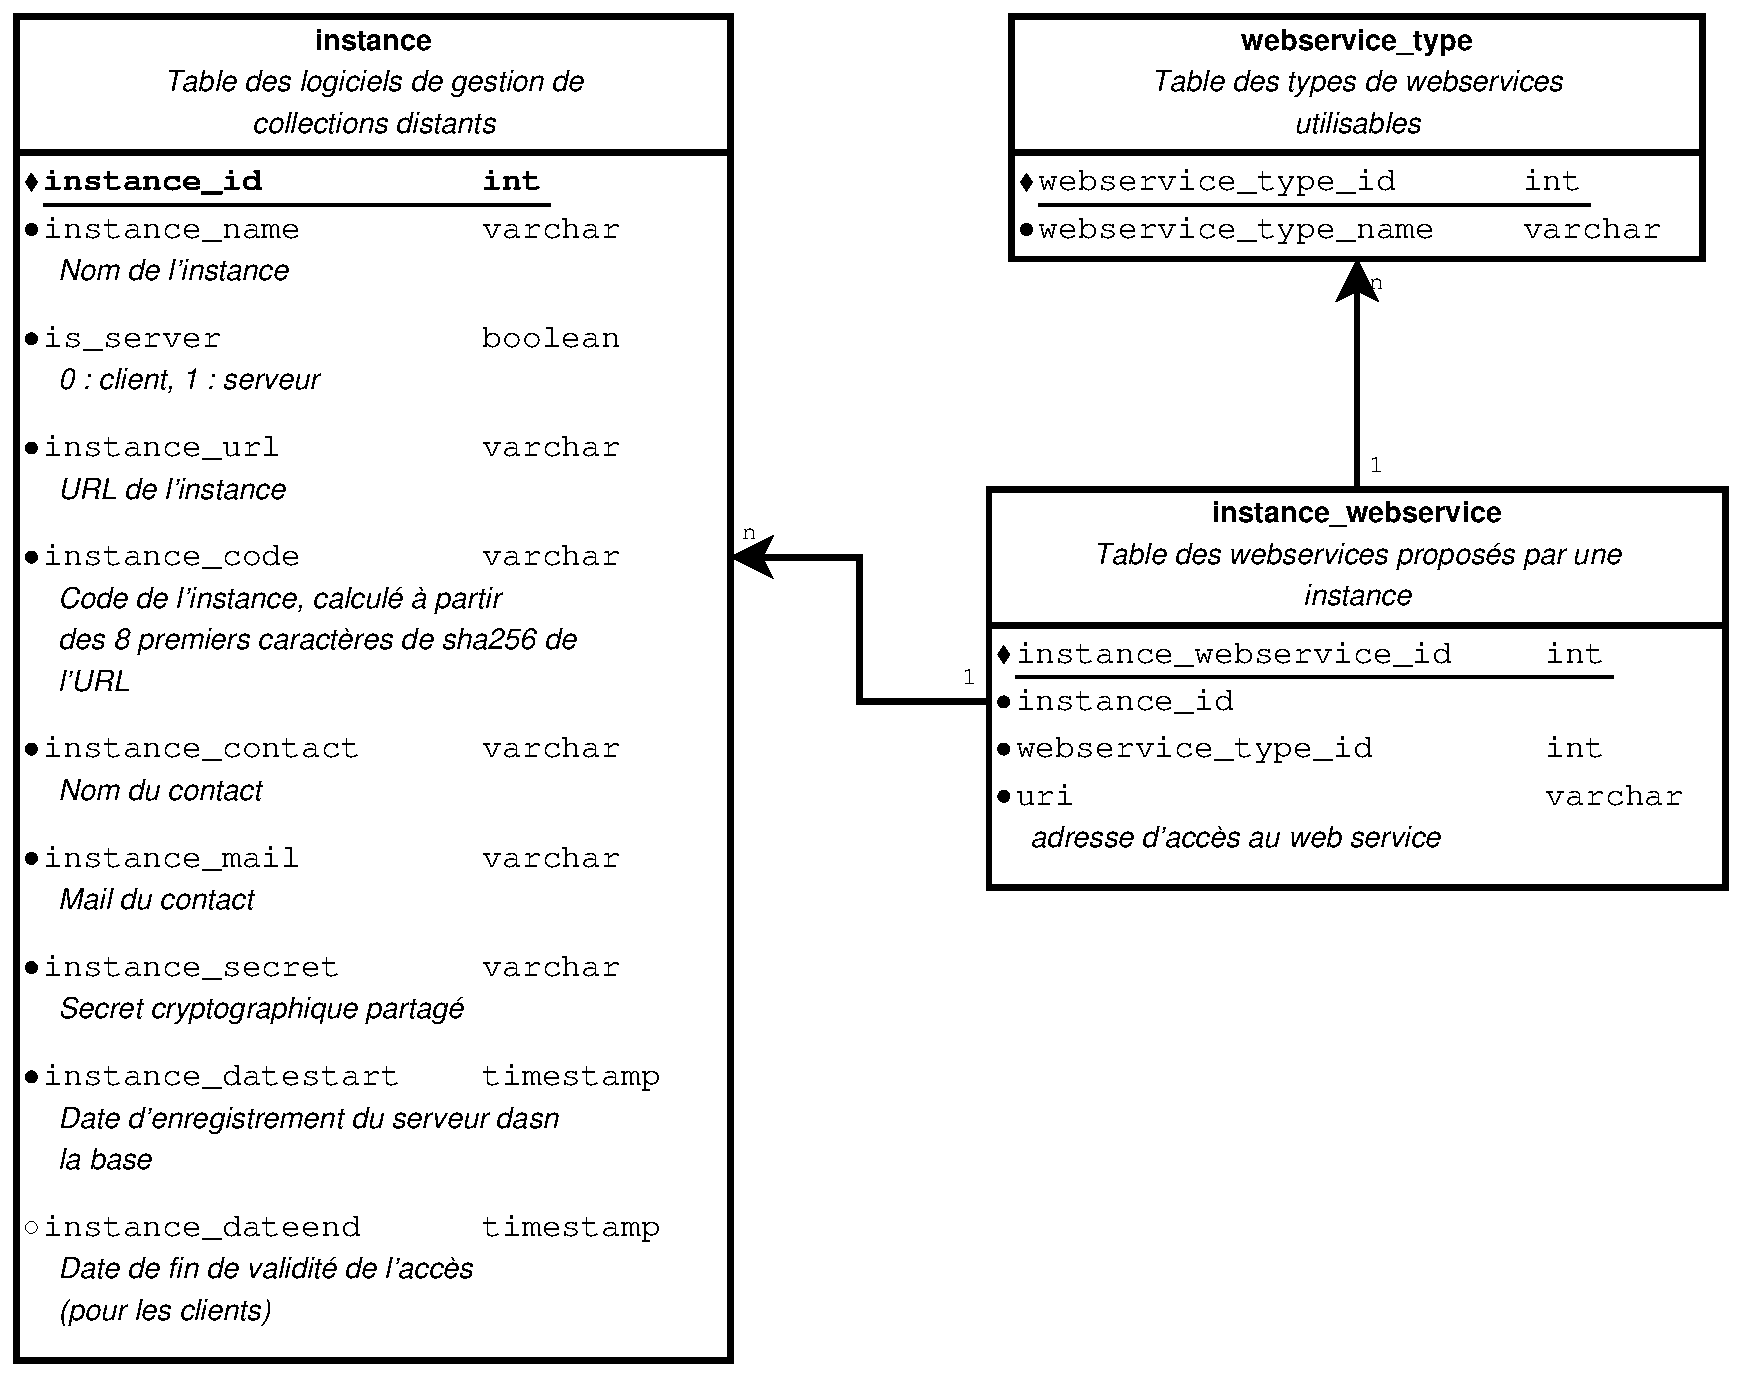
\includegraphics[width=\linewidth]{images/tables_declaration_instances}

\section{Modules et fonctions nécessaires}
\subsection{Enregistrement d'une instance distante cliente}
Ce module doit permettre d'enregistrer les données concernant une instance cliente qui sera autorisée à interroger la base locale. Il faut notamment prévoir :
\begin{itemize}
\item une fonction de génération du secret;
\item le calcul du code de l'instance, basé sur son url;
\item une fonction d'envoi d'un mail au responsable, qui contiendra un fichier json avec les informations suivantes :
\begin{itemize}
\item le code de l'instance;
\item l'url de base;
\item le secret généré;
\item la liste des services web disponibles et l'uri attachée.
\end{itemize}
\end{itemize}

Voici un exemple de la structure du fichier JSON correspondant :
\begin{lstlisting}
{
"code":"985813d1",
"url":"https://colinstance.irstea.fr",
"secret":"dad90026064f54580d24195acac1f60d2c81426e2efa9719528dee4b0ff13668",
"services":{
	{id:1,"uri":"/sw/v1/params"},
	{id:2,"uri":"/sw/v1/reference"},
	{id:3,"uri":"/sw/v1/sample_search"},
	{id:4,"uri":"/sw/v1/sample"},
	{id:5,"uri":/sw/v1/samples"}
	}
}
\end{lstlisting}

\subsection{Enregistrement d'une instance distante serveur}
Ce module doit faire l'opération inverse de la précédente. Il doit être capable de récupérer le fichier JSON transmis, pour une génération automatique dans la base de données.

\subsection{Identification d'un utilisateur distant}

Un masque de saisie dédié doit être prévu (en cas d'identification via annuaire LDAP ou base de données), pour que l'utilisateur puisse bien confirmer qu'il s'identifie dans un serveur distant.

L'appel doit contenir l'adresse de retour. Le retour doit contenir un jeton, de préférence au format JWT, chiffré avec la clé privée du serveur, avec les informations minimales suivantes :
\begin{itemize}
\item iss : origine (url du serveur);
\item exp: timestamp d'expiration;
\item uid: login de l'utilisateur.
\end{itemize}

\subsection{Module d'interrogation d'un serveur distant}
Le module doit permettre de sélectionner le serveur à interroger. Une fois le serveur sélectionné, la liste des tables de paramètres est récupérée, puis le contenu de ces tables.

FAIRE UN SCHEMA

Un masque de saisie permet de sélectionner les paramètres de recherche. Une fois les échantillons retrouvés depuis le serveur distant, il doit être possible d'en importer un dans la base locale.

Cet import va passer par une phase intermédiaire pour:
\begin{itemize}
\item associer l'échantillon au type local déclaré;
\item faire la correspondance entre les informations fournies par les tables de paramètres (identifiants secondaires, etc.). Le cas échéant, certaines informations peuvent ne pas être récupérées.
\end{itemize}
